% REV00 Tue 04 May 2021 13:55:16 WIB
% START Tue 04 May 2021 13:55:16 WIB

\chapter{XXX}

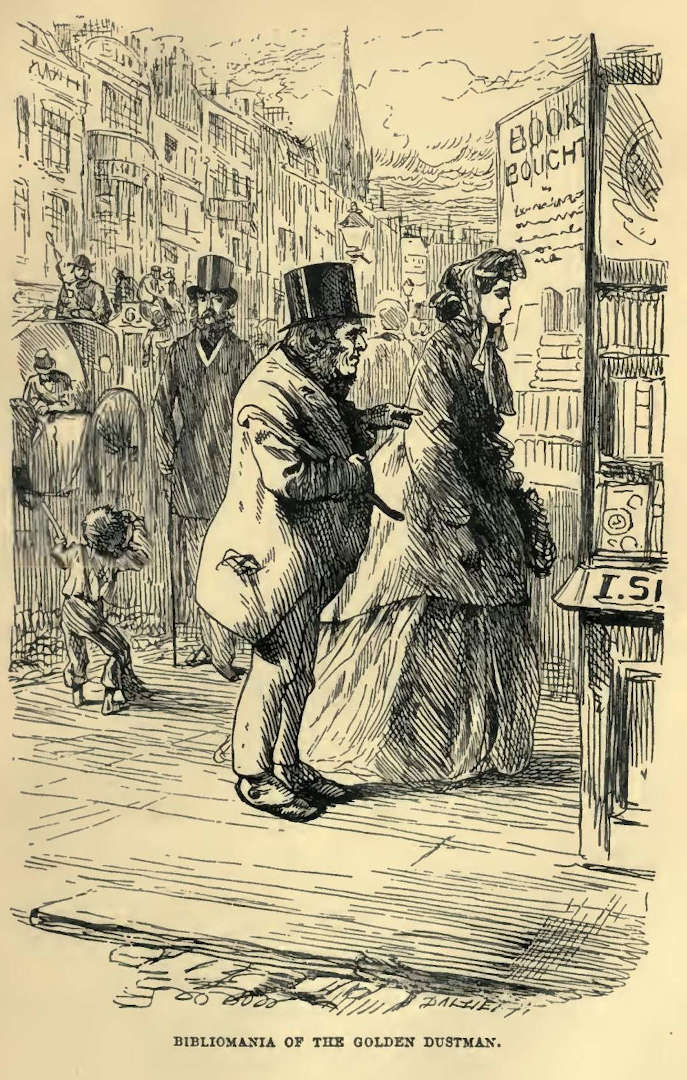
\includegraphics[scale=2.3]{03-05-01}

Chapter 9

SOMEBODY BECOMES THE SUBJECT OF A PREDICTION


‘“We give thee hearty thanks for that it hath pleased thee to deliver
this our sister out of the miseries of this sinful world.”’ So read the
Reverend Frank Milvey in a not untroubled voice, for his heart misgave
him that all was not quite right between us and our sister--or say our
sister in Law--Poor Law--and that we sometimes read these words in an
awful manner, over our Sister and our Brother too.

And Sloppy--on whom the brave deceased had never turned her back until
she ran away from him, knowing that otherwise he would not be separated
from her--Sloppy could not in his conscience as yet find the hearty
thanks required of it. Selfish in Sloppy, and yet excusable, it may be
humbly hoped, because our sister had been more than his mother.

The words were read above the ashes of Betty Higden, in a corner of a
churchyard near the river; in a churchyard so obscure that there was
nothing in it but grass-mounds, not so much as one single tombstone.
It might not be to do an unreasonably great deal for the diggers and
hewers, in a registering age, if we ticketed their graves at the common
charge; so that a new generation might know which was which: so that the
soldier, sailor, emigrant, coming home, should be able to identify the
resting-place of father, mother, playmate, or betrothed. For, we turn up
our eyes and say that we are all alike in death, and we might turn
them down and work the saying out in this world, so far. It would
be sentimental, perhaps? But how say ye, my lords and gentleman and
honourable boards, shall we not find good standing-room left for a
little sentiment, if we look into our crowds?

Near unto the Reverend Frank Milvey as he read, stood his little wife,
John Rokesmith the Secretary, and Bella Wilfer. These, over and above
Sloppy, were the mourners at the lowly grave. Not a penny had been
added to the money sewn in her dress: what her honest spirit had so long
projected, was fulfilled.

‘I’ve took it in my head,’ said Sloppy, laying it, inconsolable, against
the church door, when all was done: ‘I’ve took it in my wretched head
that I might have sometimes turned a little harder for her, and it cuts
me deep to think so now.’

The Reverend Frank Milvey, comforting Sloppy, expounded to him how the
best of us were more or less remiss in our turnings at our respective
Mangles--some of us very much so--and how we were all a halting,
failing, feeble, and inconstant crew.

‘SHE warn’t, sir,’ said Sloppy, taking this ghostly counsel rather ill,
in behalf of his late benefactress. ‘Let us speak for ourselves, sir.
She went through with whatever duty she had to do. She went through with
me, she went through with the Minders, she went through with herself,
she went through with everythink. O Mrs Higden, Mrs Higden, you was a
woman and a mother and a mangler in a million million!’

With those heartfelt words, Sloppy removed his dejected head from the
church door, and took it back to the grave in the corner, and laid it
down there, and wept alone. ‘Not a very poor grave,’ said the Reverend
Frank Milvey, brushing his hand across his eyes, ‘when it has that
homely figure on it. Richer, I think, than it could be made by most of
the sculpture in Westminster Abbey!’

They left him undisturbed, and passed out at the wicket-gate. The
water-wheel of the paper-mill was audible there, and seemed to have a
softening influence on the bright wintry scene. They had arrived but a
little while before, and Lizzie Hexam now told them the little she could
add to the letter in which she had enclosed Mr Rokesmith’s letter and
had asked for their instructions. This was merely how she had heard the
groan, and what had afterwards passed, and how she had obtained leave
for the remains to be placed in that sweet, fresh, empty store-room of
the mill from which they had just accompanied them to the churchyard,
and how the last requests had been religiously observed.

‘I could not have done it all, or nearly all, of myself,’ said Lizzie.
‘I should not have wanted the will; but I should not have had the power,
without our managing partner.’

‘Surely not the Jew who received us?’ said Mrs Milvey.

[‘My dear,’ observed her husband in parenthesis, ‘why not?’)

‘The gentleman certainly is a Jew,’ said Lizzie, ‘and the lady, his
wife, is a Jewess, and I was first brought to their notice by a Jew. But
I think there cannot be kinder people in the world.’

‘But suppose they try to convert you!’ suggested Mrs Milvey, bristling
in her good little way, as a clergyman’s wife.

‘To do what, ma’am?’ asked Lizzie, with a modest smile.

‘To make you change your religion,’ said Mrs Milvey.

Lizzie shook her head, still smiling. ‘They have never asked me what
my religion is. They asked me what my story was, and I told them. They
asked me to be industrious and faithful, and I promised to be so.
They most willingly and cheerfully do their duty to all of us who are
employed here, and we try to do ours to them. Indeed they do much more
than their duty to us, for they are wonderfully mindful of us in many
ways.’

‘It is easy to see you’re a favourite, my dear,’ said little Mrs Milvey,
not quite pleased.

‘It would be very ungrateful in me to say I am not,’ returned Lizzie,
‘for I have been already raised to a place of confidence here. But that
makes no difference in their following their own religion and leaving
all of us to ours. They never talk of theirs to us, and they never talk
of ours to us. If I was the last in the mill, it would be just the same.
They never asked me what religion that poor thing had followed.’

‘My dear,’ said Mrs Milvey, aside to the Reverend Frank, ‘I wish you
would talk to her.’

‘My dear,’ said the Reverend Frank aside to his good little wife, ‘I
think I will leave it to somebody else. The circumstances are hardly
favourable. There are plenty of talkers going about, my love, and she
will soon find one.’

While this discourse was interchanging, both Bella and the Secretary
observed Lizzie Hexam with great attention. Brought face to face for the
first time with the daughter of his supposed murderer, it was natural
that John Harmon should have his own secret reasons for a careful
scrutiny of her countenance and manner. Bella knew that Lizzie’s
father had been falsely accused of the crime which had had so great an
influence on her own life and fortunes; and her interest, though it had
no secret springs, like that of the Secretary, was equally natural. Both
had expected to see something very different from the real Lizzie Hexam,
and thus it fell out that she became the unconscious means of bringing
them together.

For, when they had walked on with her to the little house in the clean
village by the paper-mill, where Lizzie had a lodging with an elderly
couple employed in the establishment, and when Mrs Milvey and Bella
had been up to see her room and had come down, the mill bell rang.
This called Lizzie away for the time, and left the Secretary and Bella
standing rather awkwardly in the small street; Mrs Milvey being engaged
in pursuing the village children, and her investigations whether they
were in danger of becoming children of Israel; and the Reverend Frank
being engaged--to say the truth--in evading that branch of his spiritual
functions, and getting out of sight surreptitiously.

Bella at length said:

‘Hadn’t we better talk about the commission we have undertaken, Mr
Rokesmith?’

‘By all means,’ said the Secretary.

‘I suppose,’ faltered Bella, ‘that we ARE both commissioned, or we
shouldn’t both be here?’

‘I suppose so,’ was the Secretary’s answer.

‘When I proposed to come with Mr and Mrs Milvey,’ said Bella, ‘Mrs
Boffin urged me to do so, in order that I might give her my small
report--it’s not worth anything, Mr Rokesmith, except for it’s being
a woman’s--which indeed with you may be a fresh reason for it’s being
worth nothing--of Lizzie Hexam.’

‘Mr Boffin,’ said the Secretary, ‘directed me to come for the same
purpose.’

As they spoke they were leaving the little street and emerging on the
wooded landscape by the river.

‘You think well of her, Mr Rokesmith?’ pursued Bella, conscious of
making all the advances.

‘I think highly of her.’

‘I am so glad of that! Something quite refined in her beauty, is there
not?’

‘Her appearance is very striking.’

‘There is a shade of sadness upon her that is quite touching. At least
I--I am not setting up my own poor opinion, you know, Mr Rokesmith,’
said Bella, excusing and explaining herself in a pretty shy way; ‘I am
consulting you.’

‘I noticed that sadness. I hope it may not,’ said the Secretary in
a lower voice, ‘be the result of the false accusation which has been
retracted.’

When they had passed on a little further without speaking, Bella, after
stealing a glance or two at the Secretary, suddenly said:

‘Oh, Mr Rokesmith, don’t be hard with me, don’t be stern with me; be
magnanimous! I want to talk with you on equal terms.’

The Secretary as suddenly brightened, and returned: ‘Upon my honour I
had no thought but for you. I forced myself to be constrained, lest you
might misinterpret my being more natural. There. It’s gone.’

‘Thank you,’ said Bella, holding out her little hand. ‘Forgive me.’

‘No!’ cried the Secretary, eagerly. ‘Forgive ME!’ For there were tears
in her eyes, and they were prettier in his sight (though they smote him
on the heart rather reproachfully too) than any other glitter in the
world.

When they had walked a little further:

‘You were going to speak to me,’ said the Secretary, with the shadow so
long on him quite thrown off and cast away, ‘about Lizzie Hexam. So was
I going to speak to you, if I could have begun.’

‘Now that you CAN begin, sir,’ returned Bella, with a look as if she
italicized the word by putting one of her dimples under it, ‘what were
you going to say?’

‘You remember, of course, that in her short letter to Mrs Boffin--short,
but containing everything to the purpose--she stipulated that either
her name, or else her place of residence, must be kept strictly a secret
among us.’

Bella nodded Yes.

‘It is my duty to find out why she made that stipulation. I have it in
charge from Mr Boffin to discover, and I am very desirous for myself to
discover, whether that retracted accusation still leaves any stain upon
her. I mean whether it places her at any disadvantage towards any one,
even towards herself.’

‘Yes,’ said Bella, nodding thoughtfully; ‘I understand. That seems wise,
and considerate.’

‘You may not have noticed, Miss Wilfer, that she has the same kind of
interest in you, that you have in her. Just as you are attracted by her
beaut--by her appearance and manner, she is attracted by yours.’

‘I certainly have NOT noticed it,’ returned Bella, again italicizing
with the dimple, ‘and I should have given her credit for--’

The Secretary with a smile held up his hand, so plainly interposing ‘not
for better taste’, that Bella’s colour deepened over the little piece of
coquetry she was checked in.

‘And so,’ resumed the Secretary, ‘if you would speak with her alone
before we go away from here, I feel quite sure that a natural and easy
confidence would arise between you. Of course you would not be asked to
betray it; and of course you would not, if you were. But if you do not
object to put this question to her--to ascertain for us her own feeling
in this one matter--you can do so at a far greater advantage than I or
any else could. Mr Boffin is anxious on the subject. And I am,’ added
the Secretary after a moment, ‘for a special reason, very anxious.’

‘I shall be happy, Mr Rokesmith,’ returned Bella, ‘to be of the least
use; for I feel, after the serious scene of to-day, that I am useless
enough in this world.’

‘Don’t say that,’ urged the Secretary.

‘Oh, but I mean that,’ said Bella, raising her eyebrows.

‘No one is useless in this world,’ retorted the Secretary, ‘who lightens
the burden of it for any one else.’

‘But I assure you I DON’T, Mr Rokesmith,’ said Bella, half-crying.

‘Not for your father?’

‘Dear, loving, self-forgetting, easily-satisfied Pa! Oh, yes! He thinks
so.’

‘It is enough if he only thinks so,’ said the Secretary. ‘Excuse the
interruption: I don’t like to hear you depreciate yourself.’

‘But YOU once depreciated ME, sir,’ thought Bella, pouting, ‘and I hope
you may be satisfied with the consequences you brought upon your head!’
However, she said nothing to that purpose; she even said something to a
different purpose.

‘Mr Rokesmith, it seems so long since we spoke together naturally, that
I am embarrassed in approaching another subject. Mr Boffin. You know I
am very grateful to him; don’t you? You know I feel a true respect for
him, and am bound to him by the strong ties of his own generosity; now
don’t you?’

‘Unquestionably. And also that you are his favourite companion.’

‘That makes it,’ said Bella, ‘so very difficult to speak of him. But--.
Does he treat you well?’

‘You see how he treats me,’ the Secretary answered, with a patient and
yet proud air.

‘Yes, and I see it with pain,’ said Bella, very energetically.

The Secretary gave her such a radiant look, that if he had thanked her a
hundred times, he could not have said as much as the look said.

‘I see it with pain,’ repeated Bella, ‘and it often makes me miserable.
Miserable, because I cannot bear to be supposed to approve of it, or
have any indirect share in it. Miserable, because I cannot bear to be
forced to admit to myself that Fortune is spoiling Mr Boffin.’

‘Miss Wilfer,’ said the Secretary, with a beaming face, ‘if you could
know with what delight I make the discovery that Fortune isn’t spoiling
YOU, you would know that it more than compensates me for any slight at
any other hands.’

‘Oh, don’t speak of ME,’ said Bella, giving herself an impatient little
slap with her glove. ‘You don’t know me as well as--’

‘As you know yourself?’ suggested the Secretary, finding that she
stopped. ‘DO you know yourself?’

‘I know quite enough of myself,’ said Bella, with a charming air of
being inclined to give herself up as a bad job, ‘and I don’t improve
upon acquaintance. But Mr Boffin.’

‘That Mr Boffin’s manner to me, or consideration for me, is not what it
used to be,’ observed the Secretary, ‘must be admitted. It is too plain
to be denied.’

‘Are you disposed to deny it, Mr Rokesmith?’ asked Bella, with a look of
wonder.

‘Ought I not to be glad to do so, if I could: though it were only for my
own sake?’

‘Truly,’ returned Bella, ‘it must try you very much, and--you must
please promise me that you won’t take ill what I am going to add, Mr
Rokesmith?’

‘I promise it with all my heart.’

‘--And it must sometimes, I should think,’ said Bella, hesitating, ‘a
little lower you in your own estimation?’

Assenting with a movement of his head, though not at all looking as if
it did, the Secretary replied:

‘I have very strong reasons, Miss Wilfer, for bearing with the drawbacks
of my position in the house we both inhabit. Believe that they are not
all mercenary, although I have, through a series of strange fatalities,
faded out of my place in life. If what you see with such a gracious
and good sympathy is calculated to rouse my pride, there are other
considerations (and those you do not see) urging me to quiet endurance.
The latter are by far the stronger.’

‘I think I have noticed, Mr Rokesmith,’ said Bella, looking at him with
curiosity, as not quite making him out, ‘that you repress yourself, and
force yourself, to act a passive part.’

‘You are right. I repress myself and force myself to act a part. It is
not in tameness of spirit that I submit. I have a settled purpose.’

‘And a good one, I hope,’ said Bella.

‘And a good one, I hope,’ he answered, looking steadily at her.

‘Sometimes I have fancied, sir,’ said Bella, turning away her eyes,
‘that your great regard for Mrs Boffin is a very powerful motive with
you.’

‘You are right again; it is. I would do anything for her, bear anything
for her. There are no words to express how I esteem that good, good
woman.’

‘As I do too! May I ask you one thing more, Mr Rokesmith?’

‘Anything more.’

‘Of course you see that she really suffers, when Mr Boffin shows how he
is changing?’

‘I see it, every day, as you see it, and am grieved to give her pain.’

‘To give her pain?’ said Bella, repeating the phrase quickly, with her
eyebrows raised.

‘I am generally the unfortunate cause of it.’

‘Perhaps she says to you, as she often says to me, that he is the best
of men, in spite of all.’

‘I often overhear her, in her honest and beautiful devotion to him,
saying so to you,’ returned the Secretary, with the same steady look,
‘but I cannot assert that she ever says so to me.’

Bella met the steady look for a moment with a wistful, musing little
look of her own, and then, nodding her pretty head several times, like
a dimpled philosopher (of the very best school) who was moralizing on
Life, heaved a little sigh, and gave up things in general for a bad job,
as she had previously been inclined to give up herself.

But, for all that, they had a very pleasant walk. The trees were bare of
leaves, and the river was bare of water-lilies; but the sky was not bare
of its beautiful blue, and the water reflected it, and a delicious
wind ran with the stream, touching the surface crisply. Perhaps the old
mirror was never yet made by human hands, which, if all the images it
has in its time reflected could pass across its surface again, would
fail to reveal some scene of horror or distress. But the great serene
mirror of the river seemed as if it might have reproduced all it had
ever reflected between those placid banks, and brought nothing to the
light save what was peaceful, pastoral, and blooming.

So, they walked, speaking of the newly filled-up grave, and of Johnny,
and of many things. So, on their return, they met brisk Mrs Milvey
coming to seek them, with the agreeable intelligence that there was no
fear for the village children, there being a Christian school in the
village, and no worse Judaical interference with it than to plant its
garden. So, they got back to the village as Lizzie Hexam was coming from
the paper-mill, and Bella detached herself to speak with her in her own
home.

‘I am afraid it is a poor room for you,’ said Lizzie, with a smile of
welcome, as she offered the post of honour by the fireside.

‘Not so poor as you think, my dear,’ returned Bella, ‘if you knew all.’
Indeed, though attained by some wonderful winding narrow stairs, which
seemed to have been erected in a pure white chimney, and though very low
in the ceiling, and very rugged in the floor, and rather blinking as
to the proportions of its lattice window, it was a pleasanter room than
that despised chamber once at home, in which Bella had first bemoaned
the miseries of taking lodgers.

The day was closing as the two girls looked at one another by the
fireside. The dusky room was lighted by the fire. The grate might have
been the old brazier, and the glow might have been the old hollow down
by the flare.

‘It’s quite new to me,’ said Lizzie, ‘to be visited by a lady so nearly
of my own age, and so pretty, as you. It’s a pleasure to me to look at
you.’

‘I have nothing left to begin with,’ returned Bella, blushing, ‘because
I was going to say that it was a pleasure to me to look at you, Lizzie.
But we can begin without a beginning, can’t we?’

Lizzie took the pretty little hand that was held out in as pretty a
little frankness.

‘Now, dear,’ said Bella, drawing her chair a little nearer, and taking
Lizzie’s arm as if they were going out for a walk, ‘I am commissioned
with something to say, and I dare say I shall say it wrong, but I
won’t if I can help it. It is in reference to your letter to Mr and Mrs
Boffin, and this is what it is. Let me see. Oh yes! This is what it is.’

With this exordium, Bella set forth that request of Lizzie’s touching
secrecy, and delicately spoke of that false accusation and its
retraction, and asked might she beg to be informed whether it had any
bearing, near or remote, on such request. ‘I feel, my dear,’ said Bella,
quite amazing herself by the business-like manner in which she was
getting on, ‘that the subject must be a painful one to you, but I
am mixed up in it also; for--I don’t know whether you may know it or
suspect it--I am the willed-away girl who was to have been married to
the unfortunate gentleman, if he had been pleased to approve of me. So
I was dragged into the subject without my consent, and you were dragged
into it without your consent, and there is very little to choose between
us.’

‘I had no doubt,’ said Lizzie, ‘that you were the Miss Wilfer I have
often heard named. Can you tell me who my unknown friend is?’

‘Unknown friend, my dear?’ said Bella.

‘Who caused the charge against poor father to be contradicted, and sent
me the written paper.’

Bella had never heard of him. Had no notion who he was.

‘I should have been glad to thank him,’ returned Lizzie. ‘He has done a
great deal for me. I must hope that he will let me thank him some day.
You asked me has it anything to do--’

‘It or the accusation itself,’ Bella put in.

‘Yes. Has either anything to do with my wishing to live quite secret and
retired here? No.’

As Lizzie Hexam shook her head in giving this reply and as her glance
sought the fire, there was a quiet resolution in her folded hands, not
lost on Bella’s bright eyes.

‘Have you lived much alone?’ asked Bella.

‘Yes. It’s nothing new to me. I used to be always alone many hours
together, in the day and in the night, when poor father was alive.’

‘You have a brother, I have been told?’

‘I have a brother, but he is not friendly with me. He is a very good
boy though, and has raised himself by his industry. I don’t complain of
him.’

As she said it, with her eyes upon the fire-glow, there was an
instantaneous escape of distress into her face. Bella seized the moment
to touch her hand.

‘Lizzie, I wish you would tell me whether you have any friend of your
own sex and age.’

‘I have lived that lonely kind of life, that I have never had one,’ was
the answer.

‘Nor I neither,’ said Bella. ‘Not that my life has been lonely, for I
could have sometimes wished it lonelier, instead of having Ma going on
like the Tragic Muse with a face-ache in majestic corners, and Lavvy
being spiteful--though of course I am very fond of them both. I wish
you could make a friend of me, Lizzie. Do you think you could? I have
no more of what they call character, my dear, than a canary-bird, but I
know I am trustworthy.’

The wayward, playful, affectionate nature, giddy for want of the
weight of some sustaining purpose, and capricious because it was always
fluttering among little things, was yet a captivating one. To Lizzie it
was so new, so pretty, at once so womanly and so childish, that it won
her completely. And when Bella said again, ‘Do you think you could,
Lizzie?’ with her eyebrows raised, her head inquiringly on one side,
and an odd doubt about it in her own bosom, Lizzie showed beyond all
question that she thought she could.

‘Tell me, my dear,’ said Bella, ‘what is the matter, and why you live
like this.’

Lizzie presently began, by way of prelude, ‘You must have many lovers--’
when Bella checked her with a little scream of astonishment.

‘My dear, I haven’t one!’

‘Not one?’

‘Well! Perhaps one,’ said Bella. ‘I am sure I don’t know. I HAD one, but
what he may think about it at the present time I can’t say. Perhaps I
have half a one (of course I don’t count that Idiot, George Sampson).
However, never mind me. I want to hear about you.’

‘There is a certain man,’ said Lizzie, ‘a passionate and angry man, who
says he loves me, and who I must believe does love me. He is the friend
of my brother. I shrank from him within myself when my brother first
brought him to me; but the last time I saw him he terrified me more than
I can say.’ There she stopped.

‘Did you come here to escape from him, Lizzie?’

‘I came here immediately after he so alarmed me.’

‘Are you afraid of him here?’

‘I am not timid generally, but I am always afraid of him. I am afraid
to see a newspaper, or to hear a word spoken of what is done in London,
lest he should have done some violence.’

‘Then you are not afraid of him for yourself, dear?’ said Bella, after
pondering on the words.

‘I should be even that, if I met him about here. I look round for him
always, as I pass to and fro at night.’

‘Are you afraid of anything he may do to himself in London, my dear?’

‘No. He might be fierce enough even to do some violence to himself, but
I don’t think of that.’

‘Then it would almost seem, dear,’ said Bella quaintly, ‘as if there
must be somebody else?’

Lizzie put her hands before her face for a moment before replying: ‘The
words are always in my ears, and the blow he struck upon a stone wall as
he said them is always before my eyes. I have tried hard to think it
not worth remembering, but I cannot make so little of it. His hand was
trickling down with blood as he said to me, “Then I hope that I may
never kill him!’

Rather startled, Bella made and clasped a girdle of her arms round
Lizzie’s waist, and then asked quietly, in a soft voice, as they both
looked at the fire:

‘Kill him! Is this man so jealous, then?’

‘Of a gentleman,’ said Lizzie. ‘--I hardly know how to tell you--of a
gentleman far above me and my way of life, who broke father’s death to
me, and has shown an interest in me since.’

‘Does he love you?’

Lizzie shook her head.

‘Does he admire you?’

Lizzie ceased to shake her head, and pressed her hand upon her living
girdle.

‘Is it through his influence that you came here?’

‘O no! And of all the world I wouldn’t have him know that I am here, or
get the least clue where to find me.’

‘Lizzie, dear! Why?’ asked Bella, in amazement at this burst. But then
quickly added, reading Lizzie’s face: ‘No. Don’t say why. That was a
foolish question of mine. I see, I see.’

There was silence between them. Lizzie, with a drooping head, glanced
down at the glow in the fire where her first fancies had been nursed,
and her first escape made from the grim life out of which she had
plucked her brother, foreseeing her reward.

‘You know all now,’ she said, raising her eyes to Bella’s. ‘There is
nothing left out. This is my reason for living secret here, with the aid
of a good old man who is my true friend. For a short part of my life
at home with father, I knew of things--don’t ask me what--that I set my
face against, and tried to better. I don’t think I could have done more,
then, without letting my hold on father go; but they sometimes lie heavy
on my mind. By doing all for the best, I hope I may wear them out.’

‘And wear out too,’ said Bella soothingly, ‘this weakness, Lizzie, in
favour of one who is not worthy of it.’

‘No. I don’t want to wear that out,’ was the flushed reply, ‘nor do I
want to believe, nor do I believe, that he is not worthy of it. What
should I gain by that, and how much should I lose!’

Bella’s expressive little eyebrows remonstrated with the fire for some
short time before she rejoined:

‘Don’t think that I press you, Lizzie; but wouldn’t you gain in peace,
and hope, and even in freedom? Wouldn’t it be better not to live a
secret life in hiding, and not to be shut out from your natural and
wholesome prospects? Forgive my asking you, would that be no gain?’

‘Does a woman’s heart that--that has that weakness in it which you have
spoken of,’ returned Lizzie, ‘seek to gain anything?’

The question was so directly at variance with Bella’s views in life, as
set forth to her father, that she said internally, ‘There, you little
mercenary wretch! Do you hear that? Ain’t you ashamed of your self?’
and unclasped the girdle of her arms, expressly to give herself a
penitential poke in the side.

‘But you said, Lizzie,’ observed Bella, returning to her subject when
she had administered this chastisement, ‘that you would lose, besides.
Would you mind telling me what you would lose, Lizzie?’

‘I should lose some of the best recollections, best encouragements,
and best objects, that I carry through my daily life. I should lose my
belief that if I had been his equal, and he had loved me, I should have
tried with all my might to make him better and happier, as he would have
made me. I should lose almost all the value that I put upon the little
learning I have, which is all owing to him, and which I conquered the
difficulties of, that he might not think it thrown away upon me. I
should lose a kind of picture of him--or of what he might have been,
if I had been a lady, and he had loved me--which is always with me, and
which I somehow feel that I could not do a mean or a wrong thing before.
I should leave off prizing the remembrance that he has done me nothing
but good since I have known him, and that he has made a change within
me, like--like the change in the grain of these hands, which were
coarse, and cracked, and hard, and brown when I rowed on the river with
father, and are softened and made supple by this new work as you see
them now.’

They trembled, but with no weakness, as she showed them.

‘Understand me, my dear;’ thus she went on. ‘I have never dreamed of
the possibility of his being anything to me on this earth but the
kind picture that I know I could not make you understand, if the
understanding was not in your own breast already. I have no more dreamed
of the possibility of MY being his wife, than he ever has--and words
could not be stronger than that. And yet I love him. I love him so much,
and so dearly, that when I sometimes think my life may be but a weary
one, I am proud of it and glad of it. I am proud and glad to suffer
something for him, even though it is of no service to him, and he will
never know of it or care for it.’

Bella sat enchained by the deep, unselfish passion of this girl or woman
of her own age, courageously revealing itself in the confidence of her
sympathetic perception of its truth. And yet she had never experienced
anything like it, or thought of the existence of anything like it.

‘It was late upon a wretched night,’ said Lizzie, ‘when his eyes first
looked at me in my old river-side home, very different from this. His
eyes may never look at me again. I would rather that they never did; I
hope that they never may. But I would not have the light of them taken
out of my life, for anything my life can give me. I have told you
everything now, my dear. If it comes a little strange to me to have
parted with it, I am not sorry. I had no thought of ever parting with a
single word of it, a moment before you came in; but you came in, and my
mind changed.’

Bella kissed her on the cheek, and thanked her warmly for her
confidence. ‘I only wish,’ said Bella, ‘I was more deserving of it.’

‘More deserving of it?’ repeated Lizzie, with an incredulous smile.

‘I don’t mean in respect of keeping it,’ said Bella, ‘because any
one should tear me to bits before getting at a syllable of it--though
there’s no merit in that, for I am naturally as obstinate as a Pig. What
I mean is, Lizzie, that I am a mere impertinent piece of conceit, and
you shame me.’

Lizzie put up the pretty brown hair that came tumbling down, owing to
the energy with which Bella shook her head; and she remonstrated while
thus engaged, ‘My dear!’

‘Oh, it’s all very well to call me your dear,’ said Bella, with a
pettish whimper, ‘and I am glad to be called so, though I have slight
enough claim to be. But I AM such a nasty little thing!’

‘My dear!’ urged Lizzie again.

‘Such a shallow, cold, worldly, Limited little brute!’ said Bella,
bringing out her last adjective with culminating force.

‘Do you think,’ inquired Lizzie with her quiet smile, the hair being now
secured, ‘that I don’t know better?’

‘DO you know better though?’ said Bella. ‘Do you really believe you know
better? Oh, I should be so glad if you did know better, but I am so very
much afraid that I must know best!’

Lizzie asked her, laughing outright, whether she ever saw her own face
or heard her own voice?

‘I suppose so,’ returned Bella; ‘I look in the glass often enough, and I
chatter like a Magpie.’

‘I have seen your face, and heard your voice, at any rate,’ said Lizzie,
‘and they have tempted me to say to you--with a certainty of not going
wrong--what I thought I should never say to any one. Does that look
ill?’

‘No, I hope it doesn’t,’ pouted Bella, stopping herself in something
between a humoured laugh and a humoured sob.

‘I used once to see pictures in the fire,’ said Lizzie playfully, ‘to
please my brother. Shall I tell you what I see down there where the fire
is glowing?’

They had risen, and were standing on the hearth, the time being come for
separating; each had drawn an arm around the other to take leave.

‘Shall I tell you,’ asked Lizzie, ‘what I see down there?’

‘Limited little b?’ suggested Bella with her eyebrows raised.

‘A heart well worth winning, and well won. A heart that, once won, goes
through fire and water for the winner, and never changes, and is never
daunted.’

‘Girl’s heart?’ asked Bella, with accompanying eyebrows.

Lizzie nodded. ‘And the figure to which it belongs--’

‘Is yours,’ suggested Bella.

‘No. Most clearly and distinctly yours.’

So the interview terminated with pleasant words on both sides, and with
many reminders on the part of Bella that they were friends, and pledges
that she would soon come down into that part of the country again. There
with Lizzie returned to her occupation, and Bella ran over to the little
inn to rejoin her company.

‘You look rather serious, Miss Wilfer,’ was the Secretary’s first
remark.

‘I feel rather serious,’ returned Miss Wilfer.

She had nothing else to tell him but that Lizzie Hexam’s secret had
no reference whatever to the cruel charge, or its withdrawal. Oh yes
though! said Bella; she might as well mention one other thing; Lizzie
was very desirous to thank her unknown friend who had sent her the
written retractation. Was she, indeed? observed the Secretary. Ah! Bella
asked him, had he any notion who that unknown friend might be? He had no
notion whatever.

They were on the borders of Oxfordshire, so far had poor old Betty
Higden strayed. They were to return by the train presently, and, the
station being near at hand, the Reverend Frank and Mrs Frank, and Sloppy
and Bella and the Secretary, set out to walk to it. Few rustic paths are
wide enough for five, and Bella and the Secretary dropped behind.

‘Can you believe, Mr Rokesmith,’ said Bella, ‘that I feel as if whole
years had passed since I went into Lizzie Hexam’s cottage?’

‘We have crowded a good deal into the day,’ he returned, ‘and you were
much affected in the churchyard. You are over-tired.’

‘No, I am not at all tired. I have not quite expressed what I mean. I
don’t mean that I feel as if a great space of time had gone by, but that
I feel as if much had happened--to myself, you know.’

‘For good, I hope?’

‘I hope so,’ said Bella.

‘You are cold; I felt you tremble. Pray let me put this wrapper of mine
about you. May I fold it over this shoulder without injuring your dress?
Now, it will be too heavy and too long. Let me carry this end over my
arm, as you have no arm to give me.’

Yes she had though. How she got it out, in her muffled state, Heaven
knows; but she got it out somehow--there it was--and slipped it through
the Secretary’s.

‘I have had a long and interesting talk with Lizzie, Mr Rokesmith, and
she gave me her full confidence.’

‘She could not withhold it,’ said the Secretary.

‘I wonder how you come,’ said Bella, stopping short as she glanced at
him, ‘to say to me just what she said about it!’

‘I infer that it must be because I feel just as she felt about it.’

‘And how was that, do you mean to say, sir?’ asked Bella, moving again.

‘That if you were inclined to win her confidence--anybody’s
confidence--you were sure to do it.’

The railway, at this point, knowingly shutting a green eye and opening
a red one, they had to run for it. As Bella could not run easily so
wrapped up, the Secretary had to help her. When she took her opposite
place in the carriage corner, the brightness in her face was so charming
to behold, that on her exclaiming, ‘What beautiful stars and what a
glorious night!’ the Secretary said ‘Yes,’ but seemed to prefer to see
the night and the stars in the light of her lovely little countenance,
to looking out of window.

O boofer lady, fascinating boofer lady! If I were but legally executor
of Johnny’s will! If I had but the right to pay your legacy and to take
your receipt!--Something to this purpose surely mingled with the blast
of the train as it cleared the stations, all knowingly shutting up their
green eyes and opening their red ones when they prepared to let the
boofer lady pass.



